\subsection*{9.4}
In the long run, if one firm is profiting, all firms are profiting. Based off the assumptions made, this means new firms will join the market.\\
This will shift the supply curve to the right, lowering the equilibrium price. Profits will lower.\\
Firms will keep entering the industry until the profit is gone.
\par
If one firm is losing, all firms are losing. Based off the assumptions made, this means firms will leave the market.\\
This will shift the supply curve to the left, raising the equilibrium price. Losses will lower.\\
Firms will keep leaving the industry until the loss is gone.\\
In the long run, firms cannot make a profit or a loss, in the short run, you can.\\
$\pi=0$, $\pi_{\text{Accounting}}>0$. This is called the normal profit.\\
In the long run, the LRAC curve is driven down where the MC curve intersects with the minimum LRAC curve.
\begin{figure}[H]
    \centering
    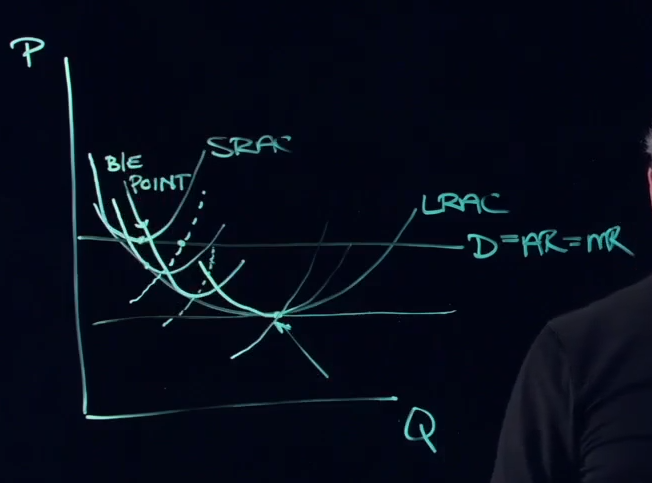
\includegraphics[width=0.5\textwidth]{./Chapter9/LongRunProfitMaximization.png}
    \caption{Long Run}
\end{figure}
Those who can quickly implement technology advances are those who profit.\\
If the taste or preferences of consumers move away from your product. Those who 
leave quickly or adapt to the price, will be able to hang on without losing money.\\
Those who are slow will lose more quickly.